\begin{figure}[h]
    \centering
    \begin{subfigure}[t]{0.3\textwidth}
        \centering
        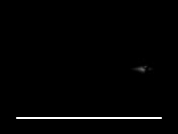
\includegraphics[width=\textwidth]{assets/5 results/ignitionFrames/16.jpg}
        \caption{\qty{1.6}{ms}}
        \label{fig:ignition_frames_16}
    \end{subfigure}
    \hfill
    \begin{subfigure}[t]{0.3\textwidth}
        \centering
        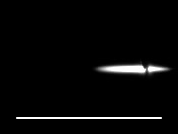
\includegraphics[width=\textwidth]{assets/5 results/ignitionFrames/17.jpg}
        \caption{\qty{1.7}{ms}}
        \label{fig:ignition_frames_17}
    \end{subfigure}
    \hfill
    \begin{subfigure}[t]{0.3\textwidth}
        \centering
        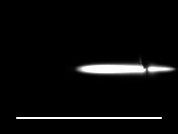
\includegraphics[width=\textwidth]{assets/5 results/ignitionFrames/18.jpg}
        \caption{\qty{1.8}{ms}}
        \label{fig:ignition_frames_18}
    \end{subfigure}
    \begin{subfigure}[t]{0.3\textwidth}
        \centering
        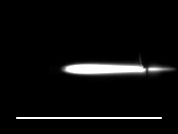
\includegraphics[width=\textwidth]{assets/5 results/ignitionFrames/19.jpg}
        \caption{\qty{1.9}{ms}}
        \label{fig:ignition_frames_19}
    \end{subfigure}
    \hfill
    \begin{subfigure}[t]{0.3\textwidth}
        \centering
        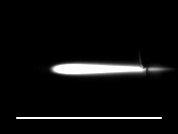
\includegraphics[width=\textwidth]{assets/5 results/ignitionFrames/20.jpg}
        \caption{\qty{2.0}{ms}}
        \label{fig:ignition_frames_20}
    \end{subfigure}
    \hfill
    \begin{subfigure}[t]{0.3\textwidth}
        \centering
        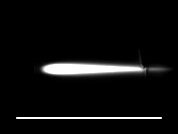
\includegraphics[width=\textwidth]{assets/5 results/ignitionFrames/21.jpg}
        \caption{\qty{2.1}{ms}}
        \label{fig:ignition_frames_21}
    \end{subfigure}
    \caption[LSP ignition via tungsten wire]{LSP ignition via tungsten wire: \qty{3080}{W}, \qty{20.29}{bar}. The white line at the bottom of each frame is \qty{10}{mm} long. \shotsettings{LSP1\_PS1}{0.1}{22}{2048}}
    \label{fig:ignition_frames}
\end{figure}